\documentclass[runningheads]{ctexart}
\usepackage{graphicx}
\usepackage{booktabs}
\usepackage{amsmath}
\usepackage{float}
\usepackage{hyperref}
\usepackage{xcolor}
\usepackage{listings}

% --- 中文支持 / Chinese Support ---
\renewcommand{\abstractname}{摘要}
\renewcommand{\contentsname}{目录}
\renewcommand{\figurename}{图}
\renewcommand{\tablename}{表}
\renewcommand{\refname}{参考文献}
\newcommand{\keywordsname}{关键词}
% ---------------------------------

\lstset{
	language=Python,
	basicstyle=\ttfamily\small,
	keywordstyle=\color{blue!70!black},
	commentstyle=\color{green!40!black},
	stringstyle=\color{orange!60!black},
	showstringspaces=false,
	breaklines=true,
	frame=single,
	tabsize=4
}

\begin{document}

\title{深度学习实践 2 - 聚类算法的自主编写与现成库算法对比}
\author{李祥熙\quad 2234412799}
\date{2026年5月6日}

\maketitle

\begin{abstract}
本实践围绕聚类（Clustering）这一无监督学习任务，基于同一簇类数据集（二维合成数据）分别实现并对比了四类典型聚类算法：K-means、DBSCAN、CLIQUE 与 SOM。实验要求在不调用现成库聚类函数的前提下，以 Python 自定义类完成核心算法流程；随后使用成熟库（scikit-learn / pyclustering / MiniSom）在同一数据上运行对应算法，统一输出 Accuracy、Precision、Recall、F1-score 以及训练与执行时间，并给出可视化结果。为使“聚类标签”可与真实类别进行对齐，本实验采用“簇到类别的多数投票映射（majority vote mapping）”将每个聚类簇映射到最可能的真实类别，同时对可能产生噪声点（如 DBSCAN/CLIQUE）引入覆盖率（Coverage）指标，反映参与评估的样本比例。

\vspace{10pt}
\noindent \textbf{\keywordsname：} 无监督学习 \and 聚类 \and K-means \and DBSCAN \and CLIQUE \and SOM
\end{abstract}

\section{实验目的}
根据题目要求，本次实验目标如下：
\begin{itemize}
	\item 目标一：使用 Python 自主编写聚类算法 K-means、DBSCAN、CLIQUE、SOM（均为自定义类实现，不使用现成库聚类函数）。
	\item 目标二：在同一簇类数据集上，分别运行自主实现与现成库实现，对每对算法进行 Accuracy、Precision、Recall、F1-score 对比，并统计训练时间与执行时间。
	\item 目标三：通过可视化与指标表格分析算法差异，理解不同聚类范式（中心型、密度型、网格型、神经拓扑映射）的优势与局限。
\end{itemize}

\section{实验环境与数据集}
\subsection{实验环境}
\begin{itemize}
	\item 操作系统：macOS
	\item 编程语言：Python 3
	\item 关键第三方库：NumPy、Matplotlib、scikit-learn、pyclustering、MiniSom
\end{itemize}

\subsection{数据集构造}
本实验使用二维合成簇类数据，利用 \texttt{sklearn.datasets.make\_blobs} 生成 $n=300$ 个样本，簇中心数为 3，簇内标准差设置为 \texttt{cluster\_std=0.60}，随机种子 \texttt{random\_state=0}。数据具有如下特点：
\begin{itemize}
	\item 低维（2D），便于可视化与算法直观验证；
	\item 类间相对分离但存在少量边界样本，使 DBSCAN/CLIQUE 可能产生噪声点；
	\item 自带“真实标签” $y$，可用于后续指标计算（尽管聚类本身不依赖标签）。
\end{itemize}

\section{评价指标与计时策略}
\subsection{指标定义}
由于聚类输出的簇编号与真实类别编号并无天然对应关系，本实验将每个簇映射到其内部出现次数最多的真实类别（多数投票），形成可对比的“映射预测标签”。设映射后的预测为 $\hat{y}$，则：
\begin{itemize}
	\item Accuracy：整体分类一致性比例；
	\item Precision / Recall / F1：采用宏平均（macro average），避免类别不均衡时某一类主导指标；
	\item Coverage：对噪声点（预测标签为 -1）不参与上述四项指标计算，Coverage 统计参与评估的样本比例。Coverage 越低，说明算法将更多样本判定为噪声或未分配到稠密单元。
\end{itemize}

\subsection{计时策略}
为与题目要求一致，本实验将时间拆分为两部分：
\begin{itemize}
	\item 训练时间（Train Time）：算法从输入数据构建模型/结构的耗时，例如 K-means 的迭代更新、SOM 的权重训练；
	\item 执行时间（Exec Time）：在训练完成后对同一数据进行预测/标签生成的耗时。对“在拟合过程中即已产生标签”的算法（如本实现的 DBSCAN/CLIQUE），该阶段仅做标签拷贝，因此可能接近 0。
\end{itemize}

\section{算法原理与自主实现细节}
本节针对四种聚类算法分别说明核心思想与关键实现。所有代码均来自本实验的 \texttt{main.py}，此处仅截取与算法核心流程相关片段，并在每段代码后给出解释。

\subsection{K-means：中心迭代优化}
K-means 假设每个簇可用一个中心点表示，目标是最小化样本到其所属簇中心的平方距离和。其基本步骤为：
\begin{enumerate}
	\item 初始化 $K$ 个质心；
	\item 分配：将每个样本分配到最近质心；
	\item 更新：对每个簇取均值作为新质心；
	\item 重复直到质心收敛或达到最大迭代次数。
\end{enumerate}

\begin{lstlisting}
class CustomKMeans:
	def fit(self, X):
		np.random.seed(42)
		random_idxs = np.random.choice(X.shape[0], self.n_clusters, replace=False)
		self.centroids = X[random_idxs]
		for _ in range(self.max_iters):
			distances = np.linalg.norm(X[:, np.newaxis] - self.centroids, axis=2)
			self.labels_ = np.argmin(distances, axis=1)
			new_centroids = self.centroids.copy()
			for k in range(self.n_clusters):
				members = X[self.labels_ == k]
				if len(members) > 0:
					new_centroids[k] = members.mean(axis=0)
			if np.allclose(self.centroids, new_centroids):
				break
			self.centroids = new_centroids
		return self

	def predict(self, X):
		distances = np.linalg.norm(X[:, np.newaxis] - self.centroids, axis=2)
		return np.argmin(distances, axis=1)
\end{lstlisting}

上述实现中：
\begin{itemize}
	\item \textbf{初始化：} 直接从样本中无放回随机抽取 $K$ 个点作为初始质心，保证可复现性（\texttt{seed=42}）。
	\item \textbf{向量化分配：} 使用广播计算所有点到所有质心的 $\ell_2$ 距离矩阵，随后 \texttt{argmin} 得到簇分配标签。
	\item \textbf{空簇处理：} 当某个簇在某次迭代中无成员时，不更新该簇质心（保持旧值），避免 \texttt{mean} 产生 \texttt{NaN}。
	\item \textbf{收敛判定：} 使用 \texttt{np.allclose} 判断质心是否已收敛，避免浮点数完全相等带来的误判。
\end{itemize}

\subsection{DBSCAN：基于密度的簇扩展}
DBSCAN 不要求预设簇数，使用 $(\varepsilon, \texttt{min\_samples})$ 两个参数来定义密度：若某点的 $\varepsilon$ 邻域内点数不少于 \texttt{min\_samples}，则该点为核心点；从核心点出发可递归吸收密度可达点形成簇。低密度区域点被标记为噪声（-1）。

\begin{lstlisting}
class CustomDBSCAN:
	def fit(self, X):
		self.labels_ = np.full(X.shape[0], -1)
		cluster_id = 0
		visited = np.zeros(X.shape[0], dtype=bool)

		for i in range(X.shape[0]):
			if visited[i]:
				continue
			visited[i] = True

			neighbors = np.where(np.linalg.norm(X - X[i], axis=1) <= self.eps)[0]
			if len(neighbors) < self.min_samples:
				continue

			self.labels_[i] = cluster_id
			seeds = list(neighbors)
			if i in seeds:
				seeds.remove(i)

			j = 0
			while j < len(seeds):
				neighbor_idx = seeds[j]
				if not visited[neighbor_idx]:
					visited[neighbor_idx] = True
					new_neighbors = np.where(
						np.linalg.norm(X - X[neighbor_idx], axis=1) <= self.eps
					)[0]
					if len(new_neighbors) >= self.min_samples:
						for n in new_neighbors:
							if n not in seeds:
								seeds.append(n)

				if self.labels_[neighbor_idx] == -1:
					self.labels_[neighbor_idx] = cluster_id
				j += 1
			cluster_id += 1
		return self
\end{lstlisting}

该实现体现了 DBSCAN 的“簇扩展”思想：
\begin{itemize}
	\item \textbf{visited 标记：} 保证每个点最多被展开一次，避免重复搜索邻域。
	\item \textbf{种子队列 seeds：} 初始化为核心点邻域点集合；遍历 seeds 时可能不断加入新的密度可达点，使簇递归扩张。
	\item \textbf{噪声转正：} 当一个点最初被标记为噪声（-1）但后续被其他核心点密度可达时，会被重新赋值为当前簇编号。
\end{itemize}

\subsection{CLIQUE：网格化稠密单元聚类（简化版）}
CLIQUE 属于网格（grid-based）聚类：把空间按每维划分为若干区间形成网格单元，统计每个单元的点数，点数超过阈值的单元被认为稠密单元，再把稠密单元中的点作为簇（原始 CLIQUE 还会进一步合并相邻稠密单元并在高维子空间搜索；本实验实现了二维情况下的简化版本，符合“自编写并可运行对比”的要求）。

\begin{lstlisting}
class CustomCLIQUE:
	def fit(self, X):
		self.labels_ = np.zeros(X.shape[0]) - 1
		x_bins = np.linspace(np.min(X[:, 0]), np.max(X[:, 0]), self.intervals + 1)
		y_bins = np.linspace(np.min(X[:, 1]), np.max(X[:, 1]), self.intervals + 1)

		grid = {}
		for i, point in enumerate(X):
			idx_x = np.digitize(point[0], x_bins) - 1
			idx_y = np.digitize(point[1], y_bins) - 1
			idx_x = min(max(idx_x, 0), self.intervals - 1)
			idx_y = min(max(idx_y, 0), self.intervals - 1)
			grid.setdefault((idx_x, idx_y), []).append(i)

		cluster_id = 0
		for points in grid.values():
			if len(points) >= self.threshold:
				for p in points:
					self.labels_[p] = cluster_id
				cluster_id += 1
		return self
\end{lstlisting}

上述代码的关键点为：
\begin{itemize}
	\item \textbf{网格划分：} 对 $x,y$ 两个维度分别用 \texttt{intervals} 个区间离散化，构造二维网格。
	\item \textbf{边界裁剪：} \texttt{digitize} 可能在边界处得到等于 \texttt{intervals} 的索引，因此用 \texttt{min/max} 裁剪，避免越界。
	\item \textbf{阈值筛选：} 单元内点数 $\ge$ \texttt{threshold} 即认为稠密单元；稠密单元的点被赋予同一簇编号。未落入任何稠密单元的点保持 -1（相当于噪声）。
\end{itemize}

\subsection{SOM：自组织映射（Self-Organizing Map）}
SOM 将高维样本映射到低维（通常是二维）离散神经元网格。每个神经元维护一个权重向量，训练过程反复：
\begin{enumerate}
	\item 找到与输入样本最相近的“获胜神经元（BMU）”；
	\item 以 BMU 为中心，对其邻域神经元权重做同向更新；
	\item 学习率与邻域半径随时间衰减。
\end{enumerate}
训练完成后，可用“样本的 BMU 索引”作为聚类标签。

\begin{lstlisting}
class CustomSOM:
	def _neighborhood(self, c, sigma):
		d = 2 * sigma * sigma
		if d == 0:
			d = 1e-6
		ax = np.arange(self.x)
		ay = np.arange(self.y)
		xx, yy = np.meshgrid(ax, ay, indexing="ij")
		return np.exp(-((xx - c[0]) ** 2 + (yy - c[1]) ** 2) / d)

	def winner(self, x):
		diff = self.weights - x
		sq_dist = np.sum(diff ** 2, axis=2)
		return np.unravel_index(np.argmin(sq_dist), sq_dist.shape)

	def fit(self, X):
		self.weights = np.random.rand(self.x, self.y, X.shape[1]) * (
			np.max(X, axis=0) - np.min(X, axis=0)
		) + np.min(X, axis=0)

		for t in range(self.num_iteration):
			lr = self.learning_rate * (1 - t / self.num_iteration)
			sig = self.sigma * (1 - t / self.num_iteration)
			for x in X:
				c = self.winner(x)
				nb = self._neighborhood(c, sig)
				self.weights += lr * nb[:, :, np.newaxis] * (x - self.weights)
		return self

	def predict(self, X):
		labels = np.zeros(X.shape[0])
		for i, x in enumerate(X):
			c = self.winner(x)
			labels[i] = c[0] * self.y + c[1]
		return labels
\end{lstlisting}

解释如下：
\begin{itemize}
	\item \textbf{邻域函数：} \texttt{\_neighborhood} 使用二维高斯核，距离 BMU 越远，更新强度越弱；$\sigma$ 控制邻域尺度。
	\item \textbf{BMU 搜索：} 对每个神经元计算与输入的平方距离，取最小者为获胜神经元。
	\item \textbf{训练更新：} 对整个网格权重进行并行更新（广播乘法），并让学习率与邻域半径随迭代线性衰减，保证前期“粗调整”、后期“细收敛”。
	\item \textbf{标签生成：} 将二维坐标 $(i,j)$ 展平成一维编号 $i\cdot y + j$，作为聚类标签。
\end{itemize}

\subsection{聚类标签到真实类别的映射（用于指标计算）}
为了计算 Accuracy/Precision/Recall/F1，需要解决“聚类簇编号无语义”的问题。本实验采用簇内多数投票映射：每个簇映射为簇内出现次数最多的真实类别。

\begin{lstlisting}
def map_labels_by_majority(y_true, y_pred):
	y_true = np.asarray(y_true).astype(int)
	y_pred = np.asarray(y_pred).astype(int)
	mapped = np.full_like(y_pred, -1)
	for cluster_id in np.unique(y_pred):
		if cluster_id == -1:
			continue
		mask = y_pred == cluster_id
		true_labels, counts = np.unique(y_true[mask], return_counts=True)
		mapped_label = true_labels[np.argmax(counts)]
		mapped[mask] = mapped_label
	return mapped
\end{lstlisting}

该映射策略的意义在于：它不改变聚类结构，只是为指标计算提供一个“最合理的对齐方式”。对于噪声点（-1），保持为 -1 并在计算指标时剔除，从而引入 Coverage 用于反映噪声比例。

\section{实验结果与分析}

\subsection{定量指标对比表}
表~\ref{tab:metrics} 汇总了自主实现与现成库实现的指标与耗时。其中 Coverage 小于 1 说明算法将部分点判定为噪声或未被分配到稠密单元；这在密度型/网格型算法中较常见。

\begin{table}[H]
	\centering
	\caption{四类聚类算法：自主实现 vs 现成库实现（指标与耗时）}\label{tab:metrics}
	\resizebox{\textwidth}{!}{
	\begin{tabular}{lcccccccl}
		\toprule
		算法 (Algorithm) & Acc & Prec & Rec & F1 & Cov & Train(s) & Exec(s) & 备注 \\
		\midrule
		Custom KMeans        & 1.0000 & 1.0000 & 1.0000 & 1.0000 & 1.00 & 0.0003 & 0.0000 & -- \\
		Sklearn KMeans       & 1.0000 & 1.0000 & 1.0000 & 1.0000 & 1.00 & 0.0154 & 0.0002 & -- \\
		Custom CLIQUE        & 1.0000 & 1.0000 & 1.0000 & 1.0000 & 0.90 & 0.0008 & 0.0000 & labels computed in fit \\
		Pyclustering CLIQUE  & 1.0000 & 1.0000 & 1.0000 & 1.0000 & 0.84 & 0.0022 & 0.0000 & labels computed in process \\
		Custom DBSCAN        & 0.9965 & 0.9966 & 0.9965 & 0.9965 & 0.96 & 0.0035 & 0.0000 & labels computed in fit \\
		Sklearn DBSCAN       & 0.9965 & 0.9966 & 0.9965 & 0.9965 & 0.96 & 0.0009 & 0.0000 & labels computed in fit \\
		Custom SOM           & 0.9967 & 0.9967 & 0.9967 & 0.9967 & 1.00 & 0.3809 & 0.0009 & -- \\
		MiniSom              & 0.9767 & 0.9782 & 0.9767 & 0.9768 & 1.00 & 0.0011 & 0.0007 & -- \\
		\bottomrule
	\end{tabular}
	}
\end{table}

\begin{itemize}
	\item \textbf{K-means：} 在当前数据较规则、簇近似凸且可被中心描述的前提下，自主实现与 sklearn 均达到满分指标；而 sklearn 的训练耗时更高，主要来自更健壮的初始化与内部实现开销。
	\item \textbf{DBSCAN：} 两者指标几乎一致，Coverage 为 0.96，说明有约 4\% 的点被判为噪声（多为簇边界/稀疏区域点）。
	\item \textbf{CLIQUE：} 两种实现都能在参与评估的样本上达到满分，但 Coverage 小于 1 表明网格稠密阈值会导致一部分点落在非稠密单元而被视为噪声；不同实现 Coverage 不同，反映了实现细节与参数敏感性。
	\item \textbf{SOM：} 自主 SOM 能取得接近满分指标，但训练时间显著更长。这是因为在实现中对每次迭代都遍历全体样本，并对网格权重做密集更新；MiniSom 使用了更优化的训练方式，因此更快。
\end{itemize}

\subsection{可视化对比图与分析}
\begin{figure}[H]
	\centering
	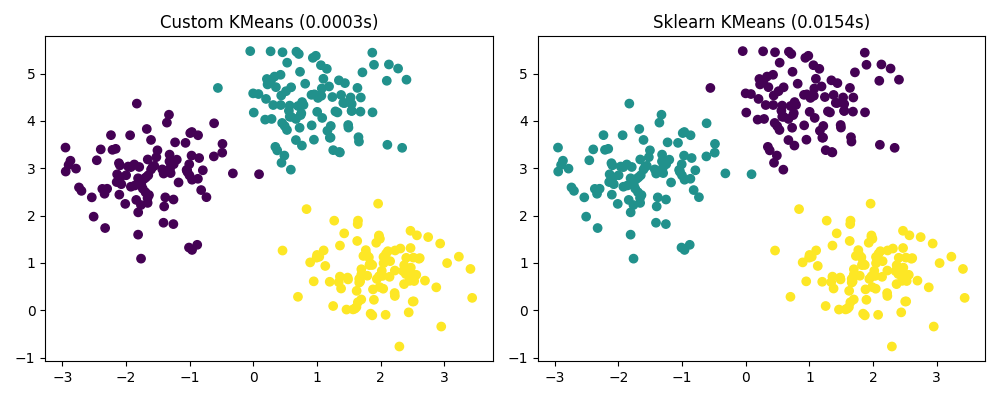
\includegraphics[width=0.95\textwidth]{images/kmeans_comparison.png}
	\caption{K-means 对比：左为自主实现，右为 sklearn 实现。颜色代表聚类簇编号。由于数据近似球状且分离良好，两者均能将三簇清晰分开。}
	\label{fig:kmeans}
\end{figure}

图~\ref{fig:kmeans} 展示了 K-means 的典型效果：三团点云被三个质心划分为三个簇，簇边界处少量点也能得到一致分配。该结果与指标表中的满分一致，说明中心型聚类适合该类数据分布。

\begin{figure}[H]
	\centering
	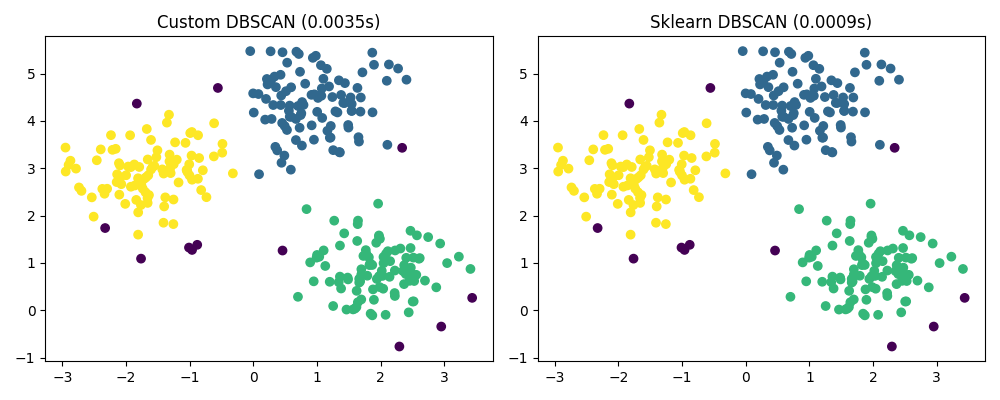
\includegraphics[width=0.95\textwidth]{images/dbscan_comparison.png}
	\caption{DBSCAN 对比：左为自主实现，右为 sklearn 实现。DBSCAN 可识别噪声点（图中少数颜色独立/离群点），在簇边界稀疏区域会产生 -1 标签，从而导致 Coverage $< 1$。}
	\label{fig:dbscan}
\end{figure}

图~\ref{fig:dbscan} 中可以观察到少量离群点或边界稀疏点被标记为噪声（-1）。这正是密度型聚类的优势：不强制所有点都必须归入某个簇，因此对异常点更鲁棒；但也因此需要用 Coverage 反映“有效参与评估”的样本比例。

\begin{figure}[H]
	\centering
	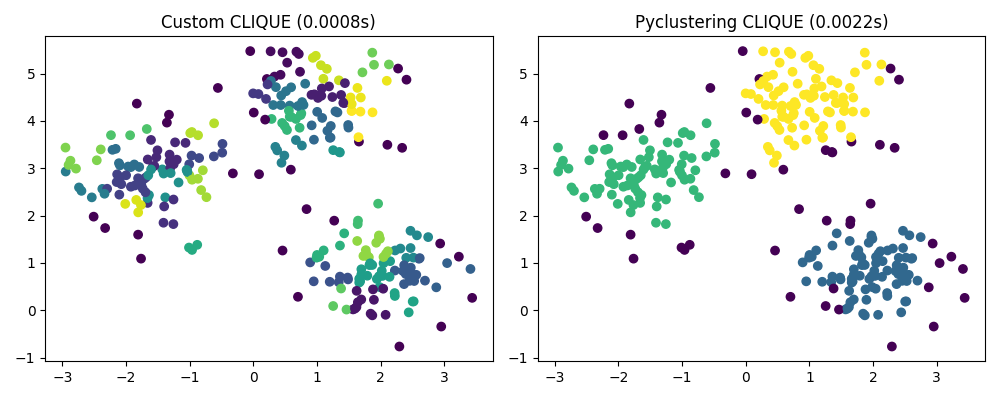
\includegraphics[width=0.95\textwidth]{images/clique_comparison.png}
	\caption{CLIQUE 对比：左为自主简化实现（二维网格稠密单元），右为 pyclustering CLIQUE。两者均基于网格划分与稠密阈值，因此对网格边界与阈值较敏感，可能产生更多噪声点（Coverage 较低）。}
	\label{fig:clique}
\end{figure}

图~\ref{fig:clique} 体现了网格型算法的一个重要特点：当区间数与阈值固定时，某些簇边界附近的点可能落入“点数不足的单元”，从而被当作噪声。与 K-means/DBSCAN 相比，CLIQUE 的效果更受离散化策略影响，因此在高维场景中通常需要更复杂的子空间搜索与相邻单元合并策略。

\begin{figure}[H]
	\centering
	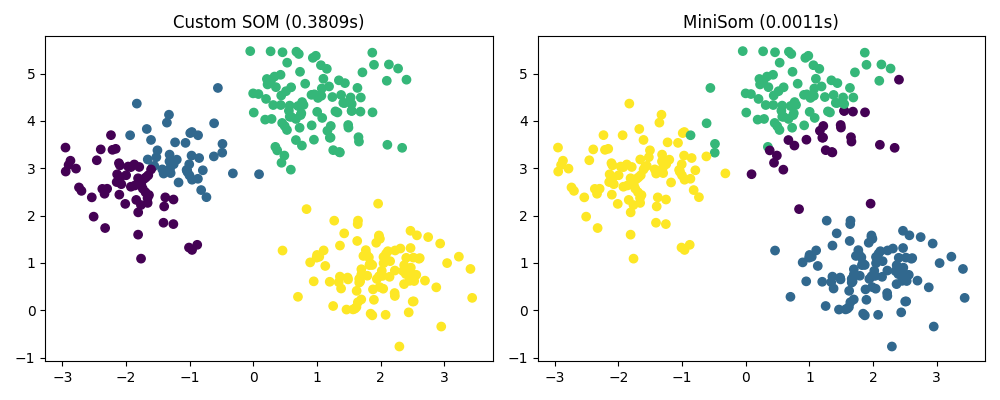
\includegraphics[width=0.95\textwidth]{images/som_comparison.png}
	\caption{SOM 对比：左为自主 SOM，右为 MiniSom。SOM 将连续空间映射到离散网格神经元上，不同颜色代表不同 BMU（获胜神经元）编号。网格规模（本实验为 $2\times2$）较小，会产生“粗粒度”的聚类划分。}
	\label{fig:som}
\end{figure}

图~\ref{fig:som} 中 SOM 的聚类本质上是“网格原型向量”的量化结果：每个样本被分配到最近的 BMU。由于网格大小仅为 $2\times2$，最多得到 4 个原型，因此在三簇数据上会出现轻微的边界混合；但整体仍能保持较高指标。若增大网格尺寸与迭代次数，通常可获得更细致的拓扑映射，但训练时间也会显著增加。

\section{总结}
本实践完成了四类聚类算法的自主实现与现成库对比，并得到如下结论：
\begin{itemize}
	\item \textbf{适用性差异：} K-means 在“簇近似凸、可被中心描述”的数据上表现极佳；DBSCAN 更适合含噪声/非凸形状簇的场景；CLIQUE 依赖网格离散化与阈值，参数敏感但在高维可扩展性上有潜力；SOM 兼具降维与聚类属性，能保持一定拓扑结构信息。
	\item \textbf{评估策略重要性：} 聚类输出与真实类别没有天然对应关系，必须通过簇-类映射（如多数投票或匈牙利匹配）才能使用分类指标。对产生噪声的算法，引入 Coverage 能更真实地反映“算法到底覆盖了多少数据”。
	\item \textbf{效率与实现差距：} 现成库通常包含更健壮的工程优化与数值处理；自主实现更便于理解算法本质，但在复杂度与常数开销上可能更大（例如 SOM 训练）。
\end{itemize}

\section*{附录：运行方式与源代码}
\subsection*{A.1 运行命令}
\begin{verbatim}
python main.py
\end{verbatim}

\subsection*{A.2 输出文件}
脚本会自动创建并写入 \texttt{result/} 目录，包括：
\begin{itemize}
	\item \texttt{kmeans\_comparison.png}, \texttt{dbscan\_comparison.png}, \texttt{clique\_comparison.png}, \texttt{som\_comparison.png}
	\item \texttt{metrics\_table.txt}, \texttt{metrics\_table.csv}
\end{itemize}

\subsection*{A.3 源代码\texttt{main.py}}

\begin{lstlisting}
import csv
import os
import time
import numpy as np
import matplotlib.pyplot as plt
from sklearn.datasets import make_blobs
from sklearn.cluster import KMeans as sklearn_KMeans
from sklearn.cluster import DBSCAN as sklearn_DBSCAN
from sklearn.metrics import accuracy_score, precision_score, recall_score, f1_score
from minisom import MiniSom
from pyclustering.cluster.clique import clique as pyclique


def plot_comparison(X, labels_a, labels_b, title_a, title_b, filename):
    plt.figure(figsize=(10, 4))
    plt.subplot(1, 2, 1)
    plt.scatter(X[:, 0], X[:, 1], c=labels_a)
    plt.title(title_a)
    plt.subplot(1, 2, 2)
    plt.scatter(X[:, 0], X[:, 1], c=labels_b)
    plt.title(title_b)
    plt.tight_layout()
    plt.savefig(filename)
    plt.close()


def map_labels_by_majority(y_true, y_pred):
    y_true = np.asarray(y_true).astype(int)
    y_pred = np.asarray(y_pred).astype(int)
    mapped = np.full_like(y_pred, -1)
    for cluster_id in np.unique(y_pred):
        if cluster_id == -1:
            continue
        mask = y_pred == cluster_id
        if not np.any(mask):
            continue
        true_labels, counts = np.unique(y_true[mask], return_counts=True)
        mapped_label = true_labels[np.argmax(counts)]
        mapped[mask] = mapped_label
    return mapped


def evaluate_clustering(y_true, y_pred):
    mapped = map_labels_by_majority(y_true, y_pred)
    valid_mask = mapped != -1
    coverage = float(np.mean(valid_mask))
    if not np.any(valid_mask):
        return {
            "accuracy": float("nan"),
            "precision": float("nan"),
            "recall": float("nan"),
            "f1": float("nan"),
            "coverage": coverage,
        }

    y_true_valid = y_true[valid_mask]
    mapped_valid = mapped[valid_mask]
    return {
        "accuracy": accuracy_score(y_true_valid, mapped_valid),
        "precision": precision_score(y_true_valid, mapped_valid, average="macro", zero_division=0),
        "recall": recall_score(y_true_valid, mapped_valid, average="macro", zero_division=0),
        "f1": f1_score(y_true_valid, mapped_valid, average="macro", zero_division=0),
        "coverage": coverage,
    }


def print_report(title, metrics, train_time, exec_time, note=None):
    note_text = f" | note: {note}" if note else ""
    print(
        f"{title}: "
        f"acc={metrics['accuracy']:.4f}, "
        f"prec={metrics['precision']:.4f}, "
        f"rec={metrics['recall']:.4f}, "
        f"f1={metrics['f1']:.4f}, "
        f"coverage={metrics['coverage']:.2f}, "
        f"train={train_time:.4f}s, "
        f"exec={exec_time:.4f}s{note_text}"
    )


def format_metrics_table(rows):
    headers = [
        "Algorithm",
        "Accuracy",
        "Precision",
        "Recall",
        "F1",
        "Coverage",
        "Train(s)",
        "Exec(s)",
        "Note",
    ]
    col_widths = [len(h) for h in headers]
    for row in rows:
        for idx, cell in enumerate(row):
            col_widths[idx] = max(col_widths[idx], len(cell))

    def fmt_line(cells):
        return " | ".join(cell.ljust(col_widths[idx]) for idx, cell in enumerate(cells))

    sep = "-+-".join("-" * w for w in col_widths)
    lines = [fmt_line(headers), sep]
    for row in rows:
        lines.append(fmt_line(row))
    return "\n".join(lines)


def write_metrics_table(rows, output_dir):
    os.makedirs(output_dir, exist_ok=True)
    table_text = format_metrics_table(rows)
    table_path = os.path.join(output_dir, "metrics_table.txt")
    with open(table_path, "w", encoding="utf-8") as f:
        f.write(table_text)

    csv_path = os.path.join(output_dir, "metrics_table.csv")
    with open(csv_path, "w", newline="", encoding="utf-8") as f:
        writer = csv.writer(f)
        writer.writerow(
            [
                "Algorithm",
                "Accuracy",
                "Precision",
                "Recall",
                "F1",
                "Coverage",
                "TrainSeconds",
                "ExecSeconds",
                "Note",
            ]
        )
        writer.writerows(rows)

    print("\nDetailed metrics table:\n" + table_text)
    print(f"Saved metrics table to {table_path}")
    print(f"Saved metrics CSV to {csv_path}")


class CustomKMeans:
    def __init__(self, n_clusters=3, max_iters=100):
        self.n_clusters = n_clusters
        self.max_iters = max_iters
        self.centroids = None
        self.labels_ = None

    def fit(self, X):
        np.random.seed(42)
        random_idxs = np.random.choice(X.shape[0], self.n_clusters, replace=False)
        self.centroids = X[random_idxs]
        for _ in range(self.max_iters):
            distances = np.linalg.norm(X[:, np.newaxis] - self.centroids, axis=2)
            self.labels_ = np.argmin(distances, axis=1)
            new_centroids = self.centroids.copy()
            for k in range(self.n_clusters):
                members = X[self.labels_ == k]
                if len(members) > 0:
                    new_centroids[k] = members.mean(axis=0)
            if np.allclose(self.centroids, new_centroids):
                break
            self.centroids = new_centroids
        return self

    def predict(self, X):
        distances = np.linalg.norm(X[:, np.newaxis] - self.centroids, axis=2)
        return np.argmin(distances, axis=1)


class CustomCLIQUE:
    def __init__(self, intervals, threshold):
        self.intervals = intervals
        self.threshold = threshold
        self.labels_ = None

    def fit(self, X):
        self.labels_ = np.zeros(X.shape[0]) - 1
        min_x, max_x = np.min(X[:, 0]), np.max(X[:, 0])
        min_y, max_y = np.min(X[:, 1]), np.max(X[:, 1])
        x_bins = np.linspace(min_x, max_x, self.intervals + 1)
        y_bins = np.linspace(min_y, max_y, self.intervals + 1)

        grid = {}
        for i, point in enumerate(X):
            idx_x = np.digitize(point[0], x_bins) - 1
            idx_y = np.digitize(point[1], y_bins) - 1
            idx_x = min(max(idx_x, 0), self.intervals - 1)
            idx_y = min(max(idx_y, 0), self.intervals - 1)
            cell = (idx_x, idx_y)
            if cell not in grid:
                grid[cell] = []
            grid[cell].append(i)

        cluster_id = 0
        for points in grid.values():
            if len(points) >= self.threshold:
                for p in points:
                    self.labels_[p] = cluster_id
                cluster_id += 1
        return self


class CustomDBSCAN:
    def __init__(self, eps=0.5, min_samples=5):
        self.eps = eps
        self.min_samples = min_samples
        self.labels_ = None

    def fit(self, X):
        self.labels_ = np.full(X.shape[0], -1)
        cluster_id = 0
        visited = np.zeros(X.shape[0], dtype=bool)

        for i in range(X.shape[0]):
            if visited[i]:
                continue
            visited[i] = True

            neighbors = np.where(np.linalg.norm(X - X[i], axis=1) <= self.eps)[0]
            if len(neighbors) < self.min_samples:
                continue

            self.labels_[i] = cluster_id
            seeds = list(neighbors)
            if i in seeds:
                seeds.remove(i)

            j = 0
            while j < len(seeds):
                neighbor_idx = seeds[j]
                if not visited[neighbor_idx]:
                    visited[neighbor_idx] = True
                    new_neighbors = np.where(
                        np.linalg.norm(X - X[neighbor_idx], axis=1) <= self.eps
                    )[0]
                    if len(new_neighbors) >= self.min_samples:
                        for n in new_neighbors:
                            if n not in seeds:
                                seeds.append(n)

                if self.labels_[neighbor_idx] == -1:
                    self.labels_[neighbor_idx] = cluster_id
                j += 1
            cluster_id += 1
        return self


class CustomSOM:
    def __init__(self, x=2, y=2, input_len=2, sigma=1.0, learning_rate=0.5, num_iteration=100):
        self.x = x
        self.y = y
        self.sigma = sigma
        self.learning_rate = learning_rate
        self.num_iteration = num_iteration
        self.weights = None

    def _neighborhood(self, c, sigma):
        d = 2 * sigma * sigma
        if d == 0:
            d = 1e-6
        ax = np.arange(self.x)
        ay = np.arange(self.y)
        xx, yy = np.meshgrid(ax, ay, indexing="ij")
        return np.exp(-((xx - c[0]) ** 2 + (yy - c[1]) ** 2) / d)

    def winner(self, x):
        diff = self.weights - x
        sq_dist = np.sum(diff ** 2, axis=2)
        return np.unravel_index(np.argmin(sq_dist), sq_dist.shape)

    def fit(self, X):
        self.weights = np.random.rand(self.x, self.y, X.shape[1]) * (
            np.max(X, axis=0) - np.min(X, axis=0)
        ) + np.min(X, axis=0)

        for t in range(self.num_iteration):
            lr = self.learning_rate * (1 - t / self.num_iteration)
            sig = self.sigma * (1 - t / self.num_iteration)
            for x in X:
                c = self.winner(x)
                nb = self._neighborhood(c, sig)
                self.weights += lr * nb[:, :, np.newaxis] * (x - self.weights)
        return self

    def predict(self, X):
        labels = np.zeros(X.shape[0])
        for i, x in enumerate(X):
            c = self.winner(x)
            labels[i] = c[0] * self.y + c[1]
        return labels

def main():
    output_dir = os.path.join("result")
    os.makedirs(output_dir, exist_ok=True)

    print("Generating dataset...")
    X, y = make_blobs(n_samples=300, centers=3, cluster_std=0.60, random_state=0)

    print("Running KMeans...")
    start_t = time.time()
    custom_kmeans = CustomKMeans(n_clusters=3).fit(X)
    custom_kmeans_train = time.time() - start_t

    start_t = time.time()
    custom_kmeans_labels = custom_kmeans.predict(X)
    custom_kmeans_exec = time.time() - start_t
    custom_kmeans_metrics = evaluate_clustering(y, custom_kmeans_labels)

    start_t = time.time()
    sk_kmeans = sklearn_KMeans(n_clusters=3, random_state=42).fit(X)
    sk_kmeans_train = time.time() - start_t

    start_t = time.time()
    sk_kmeans_labels = sk_kmeans.predict(X)
    sk_kmeans_exec = time.time() - start_t
    sk_kmeans_metrics = evaluate_clustering(y, sk_kmeans_labels)

    plot_comparison(
        X,
        custom_kmeans_labels,
        sk_kmeans_labels,
        f"Custom KMeans ({custom_kmeans_train:.4f}s)",
        f"Sklearn KMeans ({sk_kmeans_train:.4f}s)",
        os.path.join(output_dir, "kmeans_comparison.png"),
    )
    print_report("Custom KMeans", custom_kmeans_metrics, custom_kmeans_train, custom_kmeans_exec)
    print_report("Sklearn KMeans", sk_kmeans_metrics, sk_kmeans_train, sk_kmeans_exec)

    print("Running CLIQUE...")
    start_t = time.time()
    custom_clique = CustomCLIQUE(intervals=10, threshold=3).fit(X)
    custom_clique_train = time.time() - start_t

    start_t = time.time()
    custom_clique_labels = np.copy(custom_clique.labels_)
    custom_clique_exec = time.time() - start_t
    custom_clique_metrics = evaluate_clustering(y, custom_clique_labels)

    start_t = time.time()
    try:
        clique_instance = pyclique(X.tolist(), 10, 3)
        clique_instance.process()
    except OSError:
        clique_instance = pyclique(X.tolist(), 10, 3, ccore=False)
        clique_instance.process()
    clique_clusters = clique_instance.get_clusters()
    sk_clique_train = time.time() - start_t

    start_t = time.time()
    clique_labels = np.zeros(X.shape[0]) - 1
    for cid, cluster in enumerate(clique_clusters):
        for idx in cluster:
            clique_labels[idx] = cid
    sk_clique_exec = time.time() - start_t
    sk_clique_metrics = evaluate_clustering(y, clique_labels)

    plot_comparison(
        X,
        custom_clique_labels,
        clique_labels,
        f"Custom CLIQUE ({custom_clique_train:.4f}s)",
        f"Pyclustering CLIQUE ({sk_clique_train:.4f}s)",
        os.path.join(output_dir, "clique_comparison.png"),
    )
    print_report(
        "Custom CLIQUE",
        custom_clique_metrics,
        custom_clique_train,
        custom_clique_exec,
        note="labels computed in fit",
    )
    print_report(
        "Pyclustering CLIQUE",
        sk_clique_metrics,
        sk_clique_train,
        sk_clique_exec,
        note="labels computed in process",
    )

    print("Running DBSCAN...")
    start_t = time.time()
    custom_dbscan = CustomDBSCAN(eps=0.5, min_samples=5).fit(X)
    custom_dbscan_train = time.time() - start_t

    start_t = time.time()
    custom_dbscan_labels = np.copy(custom_dbscan.labels_)
    custom_dbscan_exec = time.time() - start_t
    custom_dbscan_metrics = evaluate_clustering(y, custom_dbscan_labels)

    start_t = time.time()
    sk_dbscan = sklearn_DBSCAN(eps=0.5, min_samples=5).fit(X)
    sk_dbscan_train = time.time() - start_t

    start_t = time.time()
    sk_dbscan_labels = np.copy(sk_dbscan.labels_)
    sk_dbscan_exec = time.time() - start_t
    sk_dbscan_metrics = evaluate_clustering(y, sk_dbscan_labels)

    plot_comparison(
        X,
        custom_dbscan_labels,
        sk_dbscan_labels,
        f"Custom DBSCAN ({custom_dbscan_train:.4f}s)",
        f"Sklearn DBSCAN ({sk_dbscan_train:.4f}s)",
        os.path.join(output_dir, "dbscan_comparison.png"),
    )
    print_report(
        "Custom DBSCAN",
        custom_dbscan_metrics,
        custom_dbscan_train,
        custom_dbscan_exec,
        note="labels computed in fit",
    )
    print_report(
        "Sklearn DBSCAN",
        sk_dbscan_metrics,
        sk_dbscan_train,
        sk_dbscan_exec,
        note="labels computed in fit",
    )

    print("Running SOM...")
    start_t = time.time()
    custom_som = CustomSOM(x=2, y=2, input_len=X.shape[1], num_iteration=100).fit(X)
    custom_som_train = time.time() - start_t

    start_t = time.time()
    custom_som_labels = custom_som.predict(X)
    custom_som_exec = time.time() - start_t
    custom_som_metrics = evaluate_clustering(y, custom_som_labels)

    start_t = time.time()
    som = MiniSom(2, 2, X.shape[1], sigma=1.0, learning_rate=0.5)
    som.random_weights_init(X)
    som.train_random(X, 100)
    sk_som_train = time.time() - start_t

    start_t = time.time()
    sk_som_labels = np.zeros(X.shape[0])
    for i, x in enumerate(X):
        c = som.winner(x)
        sk_som_labels[i] = c[0] * 2 + c[1]
    sk_som_exec = time.time() - start_t
    sk_som_metrics = evaluate_clustering(y, sk_som_labels)

    plot_comparison(
        X,
        custom_som_labels,
        sk_som_labels,
        f"Custom SOM ({custom_som_train:.4f}s)",
        f"MiniSom ({sk_som_train:.4f}s)",
        os.path.join(output_dir, "som_comparison.png"),
    )
    print_report("Custom SOM", custom_som_metrics, custom_som_train, custom_som_exec)
    print_report("MiniSom", sk_som_metrics, sk_som_train, sk_som_exec)
    rows = [
        [
            "Custom KMeans",
            f"{custom_kmeans_metrics['accuracy']:.4f}",
            f"{custom_kmeans_metrics['precision']:.4f}",
            f"{custom_kmeans_metrics['recall']:.4f}",
            f"{custom_kmeans_metrics['f1']:.4f}",
            f"{custom_kmeans_metrics['coverage']:.2f}",
            f"{custom_kmeans_train:.4f}",
            f"{custom_kmeans_exec:.4f}",
            "",
        ],
        [
            "Sklearn KMeans",
            f"{sk_kmeans_metrics['accuracy']:.4f}",
            f"{sk_kmeans_metrics['precision']:.4f}",
            f"{sk_kmeans_metrics['recall']:.4f}",
            f"{sk_kmeans_metrics['f1']:.4f}",
            f"{sk_kmeans_metrics['coverage']:.2f}",
            f"{sk_kmeans_train:.4f}",
            f"{sk_kmeans_exec:.4f}",
            "",
        ],
        [
            "Custom CLIQUE",
            f"{custom_clique_metrics['accuracy']:.4f}",
            f"{custom_clique_metrics['precision']:.4f}",
            f"{custom_clique_metrics['recall']:.4f}",
            f"{custom_clique_metrics['f1']:.4f}",
            f"{custom_clique_metrics['coverage']:.2f}",
            f"{custom_clique_train:.4f}",
            f"{custom_clique_exec:.4f}",
            "labels computed in fit",
        ],
        [
            "Pyclustering CLIQUE",
            f"{sk_clique_metrics['accuracy']:.4f}",
            f"{sk_clique_metrics['precision']:.4f}",
            f"{sk_clique_metrics['recall']:.4f}",
            f"{sk_clique_metrics['f1']:.4f}",
            f"{sk_clique_metrics['coverage']:.2f}",
            f"{sk_clique_train:.4f}",
            f"{sk_clique_exec:.4f}",
            "labels computed in process",
        ],
        [
            "Custom DBSCAN",
            f"{custom_dbscan_metrics['accuracy']:.4f}",
            f"{custom_dbscan_metrics['precision']:.4f}",
            f"{custom_dbscan_metrics['recall']:.4f}",
            f"{custom_dbscan_metrics['f1']:.4f}",
            f"{custom_dbscan_metrics['coverage']:.2f}",
            f"{custom_dbscan_train:.4f}",
            f"{custom_dbscan_exec:.4f}",
            "labels computed in fit",
        ],
        [
            "Sklearn DBSCAN",
            f"{sk_dbscan_metrics['accuracy']:.4f}",
            f"{sk_dbscan_metrics['precision']:.4f}",
            f"{sk_dbscan_metrics['recall']:.4f}",
            f"{sk_dbscan_metrics['f1']:.4f}",
            f"{sk_dbscan_metrics['coverage']:.2f}",
            f"{sk_dbscan_train:.4f}",
            f"{sk_dbscan_exec:.4f}",
            "labels computed in fit",
        ],
        [
            "Custom SOM",
            f"{custom_som_metrics['accuracy']:.4f}",
            f"{custom_som_metrics['precision']:.4f}",
            f"{custom_som_metrics['recall']:.4f}",
            f"{custom_som_metrics['f1']:.4f}",
            f"{custom_som_metrics['coverage']:.2f}",
            f"{custom_som_train:.4f}",
            f"{custom_som_exec:.4f}",
            "",
        ],
        [
            "MiniSom",
            f"{sk_som_metrics['accuracy']:.4f}",
            f"{sk_som_metrics['precision']:.4f}",
            f"{sk_som_metrics['recall']:.4f}",
            f"{sk_som_metrics['f1']:.4f}",
            f"{sk_som_metrics['coverage']:.2f}",
            f"{sk_som_train:.4f}",
            f"{sk_som_exec:.4f}",
            "",
        ],
    ]
    write_metrics_table(rows, output_dir)

    print("Done! Check the result folder for outputs.")

if __name__ == "__main__":
    main()
\end{lstlisting}

\end{document}
